% context: markscheme (official solutions) for 2-2CW_Average-velocity
% topic: average speed vs average velocity, instantaneous velocity as the limit of
%        shorter intervals, average velocity of each leg of a path on a grid
% convention: answers in bold; "=" joins exact equalities, "\approx" introduces a
%        rounded value; velocity always carries a sign or a direction
\documentclass[12pt, twoside]{article}
%\documentclass[12pt, twoside]{article}
\usepackage[letterpaper, margin=1in, headsep=0.2in]{geometry}
\setlength{\headheight}{0.6in}
%\usepackage[english]{babel}
\usepackage[utf8]{inputenc}
\usepackage{microtype}
\usepackage{amsmath}
\usepackage{amssymb}
%\usepackage{amsfonts}
\usepackage[nomessages]{fp} %\FPeval{\var-name}{2*sin(pi/6)}
\usepackage{siunitx} %units in math. eg 20\milli\meter
\usepackage{yhmath} % for arcs, overparenth command
\usepackage{tikz} %graphics
\usetikzlibrary{quotes, angles, arrows, arrows.meta}
\usepackage{graphicx} %consider setting \graphicspath{{images/}}
\usepackage{parskip} %no paragraph indent
\usepackage{enumitem}
\usepackage{multicol}
\usepackage{venndiagram}

\usepackage{fancyhdr}
\pagestyle{fancy}
\fancyhf{}
\renewcommand{\headrulewidth}{0pt} % disable the underline of the header
\raggedbottom
\hfuzz=2mm %suppresses overfull box warnings

\usepackage{hyperref}
\usepackage{float}
\setlength{\parskip}{0.2\baselineskip}

\title{Physics}
\author{Chris Huson}
\date{October 2026}

\fancyhead[LE]{\thepage}
\fancyhead[RO]{\thepage}
\fancyhead[LO]{La Scuola d'Italia / Huson / Physics \\* 16 October 2026}

\begin{document}

\subsubsection*{2.2 Classwork: Average and Instantaneous Velocity Solutions}

\begin{enumerate}[itemsep=0.4cm]

\item Swimming.
  \begin{enumerate}[itemsep=0.2cm]
    \item Average speed $= \dfrac{50~\text{m}}{20.91~\text{s}} = 2.3912\ldots
      \approx \mathbf{2.391~\textbf{m/s}}$. \quad Average velocity
      $\approx \mathbf{2.391~\textbf{m/s}}$ \textbf{down the pool}.
    \item Average speed $= \dfrac{100~\text{m}}{46.40~\text{s}} = 2.1551\ldots
      \approx \mathbf{2.155~\textbf{m/s}}$. \quad Average velocity
      $= \dfrac{0~\text{m}}{46.40~\text{s}} = \mathbf{0}$.
  \end{enumerate}
  \emph{In one straight length, speed and velocity agree. Back at the starting wall the
  displacement is zero, so the average velocity is zero however hard the swimmer
  worked. Four significant figures come from the times; the distances are exact.}

\item Hallway walk, east positive.
  \begin{enumerate}[itemsep=0.2cm]
    \item Leg 1: $\dfrac{+8.0~\text{m}}{4.0~\text{s}} = \mathbf{+2.0~\textbf{m/s}}$
      \quad Leg 2: $\dfrac{-5.0~\text{m}}{5.0~\text{s}} = \mathbf{-1.0~\textbf{m/s}}$
      \quad Leg 3: $\dfrac{-7.0~\text{m}}{5.0~\text{s}} = \mathbf{-1.4~\textbf{m/s}}$
    \item Total time $= 4.0 + 5.0 + 5.0 = 14.0$ s; distance $= 8.0 + 5.0 + 7.0 = 20.0$ m;
      displacement $= 8.0 - 5.0 - 7.0 = -4.0$ m.

      Average speed $= \dfrac{20.0~\text{m}}{14.0~\text{s}} = 1.428\ldots
      \approx \mathbf{1.4~\textbf{m/s}}$ \quad
      Average velocity $= \dfrac{-4.0~\text{m}}{14.0~\text{s}} = -0.2857\ldots
      \approx \mathbf{-0.29~\textbf{m/s}}$ \textbf{(west)}

      \emph{The walk went back over its own path, so most of the distance cancels in
      the displacement. Accept 1.43 m/s and $-0.286$ m/s. Do not accept averaging the
      three leg velocities: $(2.0 - 1.0 - 1.4) \div 3$ ignores that the legs take
      different times.}
  \end{enumerate}

\item Frecciarossa.
  \begin{enumerate}[itemsep=0.2cm]
    \item The speed is wanted in km/h, so first write the time in hours:
      $2~\text{h}~59~\text{min} = 2 + \dfrac{59}{60} = 2.98333\ldots~\text{h}$.

      $\bar{v} = \dfrac{570~\text{km}}{2.98333\ldots~\text{h}} = 191.06\ldots
      \approx \mathbf{191~\textbf{km/h}}$

      \emph{Accept 190 km/h: ``about 570 km'' supports two or three figures. Do not
      accept $570 \div 2.59$: 2 h 59 min is not 2.59 h.}
    \item \textbf{Instantaneous.} \emph{The display shows the speed at that moment.
      The average is lower because the train starts from rest in Rome, slows to stop
      in Milan, and runs more slowly on the approaches to both cities and on curves.
      Any one sound reason earns the mark.}
  \end{enumerate}

\newpage

\item Instantaneous velocity.
  \begin{enumerate}[itemsep=0.25cm]
    \item \renewcommand{\arraystretch}{1.35}
      \begin{tabular}[t]{| c | c | c | c |}
        \hline
        Interval & $\Delta t$ (s) & $\Delta x$ (m) & $\bar{v}$ (m/s) \\ \hline
        1.00 s to 2.00 s & 1.00 & 0.750 & \textbf{0.750} \\ \hline
        1.00 s to 1.50 s & 0.50 & 0.313 & \textbf{0.626} \\ \hline
        1.00 s to 1.10 s & 0.10 & 0.053 & \textbf{0.53} \\ \hline
        1.00 s to 1.05 s & 0.05 & 0.026 & \textbf{0.52} \\ \hline
      \end{tabular}
    \item \textbf{About 0.50 m/s.} \emph{The averages fall toward 0.5 as the interval
      shrinks. The data were made from $x = 0.25\,t^2$, for which the exact value at
      $t = 1.00$ s is 0.500 m/s.}
    \item \emph{Positions are recorded to the nearest millimeter. Over 0.05 s the cart
      moves only 26 mm, so $\Delta x$ has just two significant figures; over 0.01 s it
      would move about 5 mm, one significant figure, and $\bar{v}$ would be no better
      than ``about 0.5''. The measurement precision runs out before the interval does.
      Also accept: the data only has points every 0.05 s.}
  \end{enumerate}

\item Soccer drill, east $+x$, north $+y$.

  \begin{minipage}[t]{0.56\linewidth}
    \vspace{0pt}
    \begin{enumerate}[itemsep=0.25cm]
      \item Path drawn head to tail: $(0,0) \to (6,0) \to (6,4) \to (0,4)$.
      \item Leg 1: $\dfrac{6.0~\text{m}}{2.0~\text{s}} = \mathbf{3.0~\textbf{m/s east}}$
        \\[0.2cm]
        Leg 2: $\dfrac{4.0~\text{m}}{2.0~\text{s}} = \mathbf{2.0~\textbf{m/s north}}$
        \\[0.2cm]
        Leg 3: $\dfrac{6.0~\text{m}}{3.0~\text{s}} = \mathbf{2.0~\textbf{m/s west}}$

        \emph{Legs 2 and 3 have the same speed but different velocities: the arrows
        point different ways.}
      \item Distance $= 6.0 + 4.0 + 6.0 = 16.0$ m in $7.0$ s.

        Average speed $= \dfrac{16.0~\text{m}}{7.0~\text{s}} = 2.285\ldots
        \approx \mathbf{2.3~\textbf{m/s}}$

        The player finishes at $(0,4)$, so the displacement is $4.0$ m north.

        Average velocity $= \dfrac{4.0~\text{m}}{7.0~\text{s}} = 0.5714\ldots
        \approx \mathbf{0.57~\textbf{m/s north}}$
    \end{enumerate}
  \end{minipage}
  \hfill
  \begin{minipage}[t]{0.4\linewidth}
    \vspace{0pt}
    \centering
    \begin{tikzpicture}[scale=0.45]
      \draw[gray!40, thin, step=1] (-1,-1) grid (8,5);
      \draw[->, thick] (-1.3,0) -- (8.6,0) node[right]{\small $x$};
      \draw[->, thick] (0,-1.3) -- (0,5.6) node[above]{\small $y$};
      \foreach \x in {2,4,6,8} \node[below] at (\x,0) {\scriptsize \x};
      \foreach \y in {2,4} \node[left] at (0,\y) {\scriptsize \y};
      \node[below] at (3.5,-1.3) {\small path: 1 square = 1 m};
      \draw[->, very thick] (0,0) -- (6,0) node[midway, above]{\small 1};
      \draw[->, very thick] (6,0) -- (6,4) node[midway, right]{\small 2};
      \draw[->, very thick] (6,4) -- (0,4) node[midway, above]{\small 3};
    \end{tikzpicture}

    \vspace{0.15cm}
    \begin{tikzpicture}[scale=0.45]
      \draw[gray!40, thin, step=1] (-4,-1) grid (4,3);
      \draw[->, thick] (-4.3,0) -- (4.6,0) node[right]{\small $x$};
      \draw[->, thick] (0,-1.3) -- (0,3.6) node[above]{\small $y$};
      \foreach \x in {-4,-2,2,4} \node[below] at (\x,0) {\scriptsize \x};
      \foreach \y in {2} \node[left] at (0,\y) {\scriptsize \y};
      \node[below] at (0,-1.3) {\small velocity: 1 square = 1 m/s};
      \draw[->, very thick] (0,0) -- (3,0) node[midway, above]{\small 1};
      \draw[->, very thick] (0,0) -- (0,2) node[midway, right]{\small 2};
      \draw[->, very thick] (0,0) -- (-2,0) node[midway, above]{\small 3};
    \end{tikzpicture}
  \end{minipage}

  \vspace{0.3cm}
  \emph{Reading the finish point off the grid is all that is needed here; adding
  vectors in two dimensions comes later. Accept 2.29 m/s and 0.571 m/s north. The
  average velocity is small because the player ends only 4 m from the start.}

\end{enumerate}
\end{document}
